\documentclass{standalone}
\usepackage{tikz}
\usetikzlibrary{3d}

\begin{document}

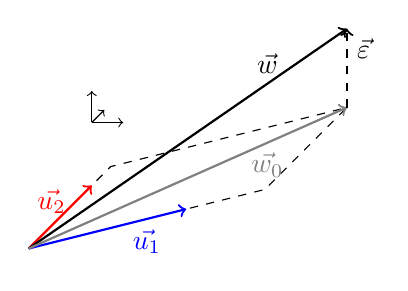
\begin{tikzpicture}[x={(2cm,0cm)}, z={(0cm,2cm)}, y={(0.8cm,0.8cm)}]

  % Definice bodů

\begin{scope}[x={(2cm,0.5cm)}]

  
\coordinate (A) at (1,0,0);
\coordinate (B) at (0,1,0);
\coordinate (C) at (1.5,1.3,0.5); % Třetí vektor, který neleží v rovině
\coordinate (C0) at (1.5,1.3,0); 


% Vykreslení vektorů
\draw[-, dashed] (0,0,0) -- (1.5,0,0) -- (1.5,1.3,0) -- (0,1.3,0) --(0,0,0);
\draw[->,thick,blue] (0,0,0) -- node[near end, below] {$\vec{u_1}$} (A);
\draw[->,thick,red] (0,0,0) -- node[near end, left] {$\vec{u_2}$} (B);
\draw[->,thick] (0,0,0) -- node[near end,above] {$\vec{w}$} (C);
\draw[->,thick,gray] (0,0,0) --  (C0) node[near end, below] {$\vec{w_0}$};

\draw[->,thick, dashed] (C0) -- node[near end, right]{$\vec\varepsilon$} (C);

\end{scope}
% Popisky os
\begin{scope}[shift={(0.4,0,.8)}, scale=0.2]
\draw[->] (0,0,0) -- (1,0,0);
\draw[->] (0,0,0) -- (0,1,0);
\draw[->] (0,0,0) -- (0,0,1);
\end{scope}
\end{tikzpicture}

\end{document}
